We apply the results from \autoref{chapter: thermodynamics} to study the properties of pion stars.

\section{Leading-order results}

We start with the most simple model, using the leading order equation of state with $e = 0$.
We can gain some insights by reviewing the units of the problem.
The characteristic mass and length, as discussed in \autoref{section: TOV equation}, are found by setting $k_1 = k_2 = k_3 = 1$.
These are the dimensionless constants of the TOV equation, \autoref{dimensionless constants TOV}.
At leading order, the bare constants $f$ and $\bar m$ are related to physical constants by $f = f_\pi$ and $m = m_\pi$, the pion decay constant and the pion mass.
Using the values for $f_\pi$ and $m_\pi$ as given in \autoref{section: units} and reinstating $c$ and $\hbar$, these quantities are give in by
%
\begin{align}
    u_0 & =m_\pi^2 f_\pi^2 \frac{c}{\hbar^3}
    = 3.216\cdot 10^{33} \, \text{J}\,\text{m}^{-3}, \\
    m_0 & = \frac{c^4}{\sqrt{\frac{4 \pi}{ 3} u_0 G^3}} = 64.21\, M_\odot, \\
    r_0 & = \frac{G}{c^2} m_0 = 94.79 \, \text{km}.
\end{align}
%
We, therefore, expect both the radius and mass of the pion star to be around one order of magnitude larger than the star made up of cold neutrons.
\todo[inline]{Can we make a better argument by setting gravitational + internal energy equal 0?}

\subsection{Limiting radius}

We found that the non-relativisitc limit of the equation of state is $\tilde p =8^{-1} \tilde u^2$, i.e., it is a polytrope with $\gamma = 2$.
As discussed in \autoref{subsection: Newtonian limit and polytropes}, this corresponds to a situation where the radius of the star is independent of the central pressure, at least in the Newtonian limit of gravity.
When simulating the Newtonian, non-relativistic limit of the pion star, we should expect the radius to be constant.
From \autoref{Radius polytrope}, the radius is $R = C \xi_1$, where
%
\begin{equation}
    C = \frac{1}{\sqrt{4(4\pi ) G u_0}} = \frac{1}{\sqrt{12}}r_0,
\end{equation}
%
and $\xi_1$ is the root of the Lane-Emden function $\theta(\xi)$ for polytrope index $n=1$, the solution to
%
\begin{equation}
    \theta'' + \frac{2}{\xi} \theta' + \theta = 0.
\end{equation}
%
By substituting $\theta$ for its power series expansion, $\theta = \sum_n a_n \xi^n$, we get
%
\begin{equation}
    \sum_n \left[ (n+2)(n+1) a_{n+2} + 2(n+1) a_{n+1} \xi^{-1} + a_n \right] \xi^n = 0.
\end{equation}
%
This must be obeyed for arbitrary $\xi$.
We therefore get the recursion relation $a_{n+2} = - a_n / (n+1)(n+2)$.
With our boundary condition, the solution is
%
\begin{equation}
    \theta(\xi) = \frac{\sin(\xi)}{\xi},
\end{equation}
%
and the first root is therefore $\xi_1 = \pi$.
With this, we get a closed-form expression for the stellar radius of this non-relativistic and Newtonian limit---which we expect the full theory to approach as the central pressure decreases---namely
%
\begin{equation}
    \label{radius pion star nr limit}
    R = \frac{\pi}{\sqrt{12}} r_0 = 85.97 \, \text{km}.
\end{equation}


\subsection{Results}

The code used for obtaining numerical results is discussed in \autoref{appendix: code}.

\autoref{fig: pressure and mass for pion star} show the pressure and mass as a function of radius for varying values of central pressure.
The quantities are normalized to the stellar radius, stellar mass, and central pressure, respectively.
The black dashed line corresponds to the configuration with the maximum mass.
We see that both the pressure and mass distribution are very similar for stars with a mass less than the maximum.
As the central pressure increase beyond that of the star with maximum mass, the pressure gradient close to the center grows sharply.
This is similar to what we saw in the case of an incompressible fluid, \autoref{subsection: incompressible fluid}.

\begin{figure}[!h]
    \centering
    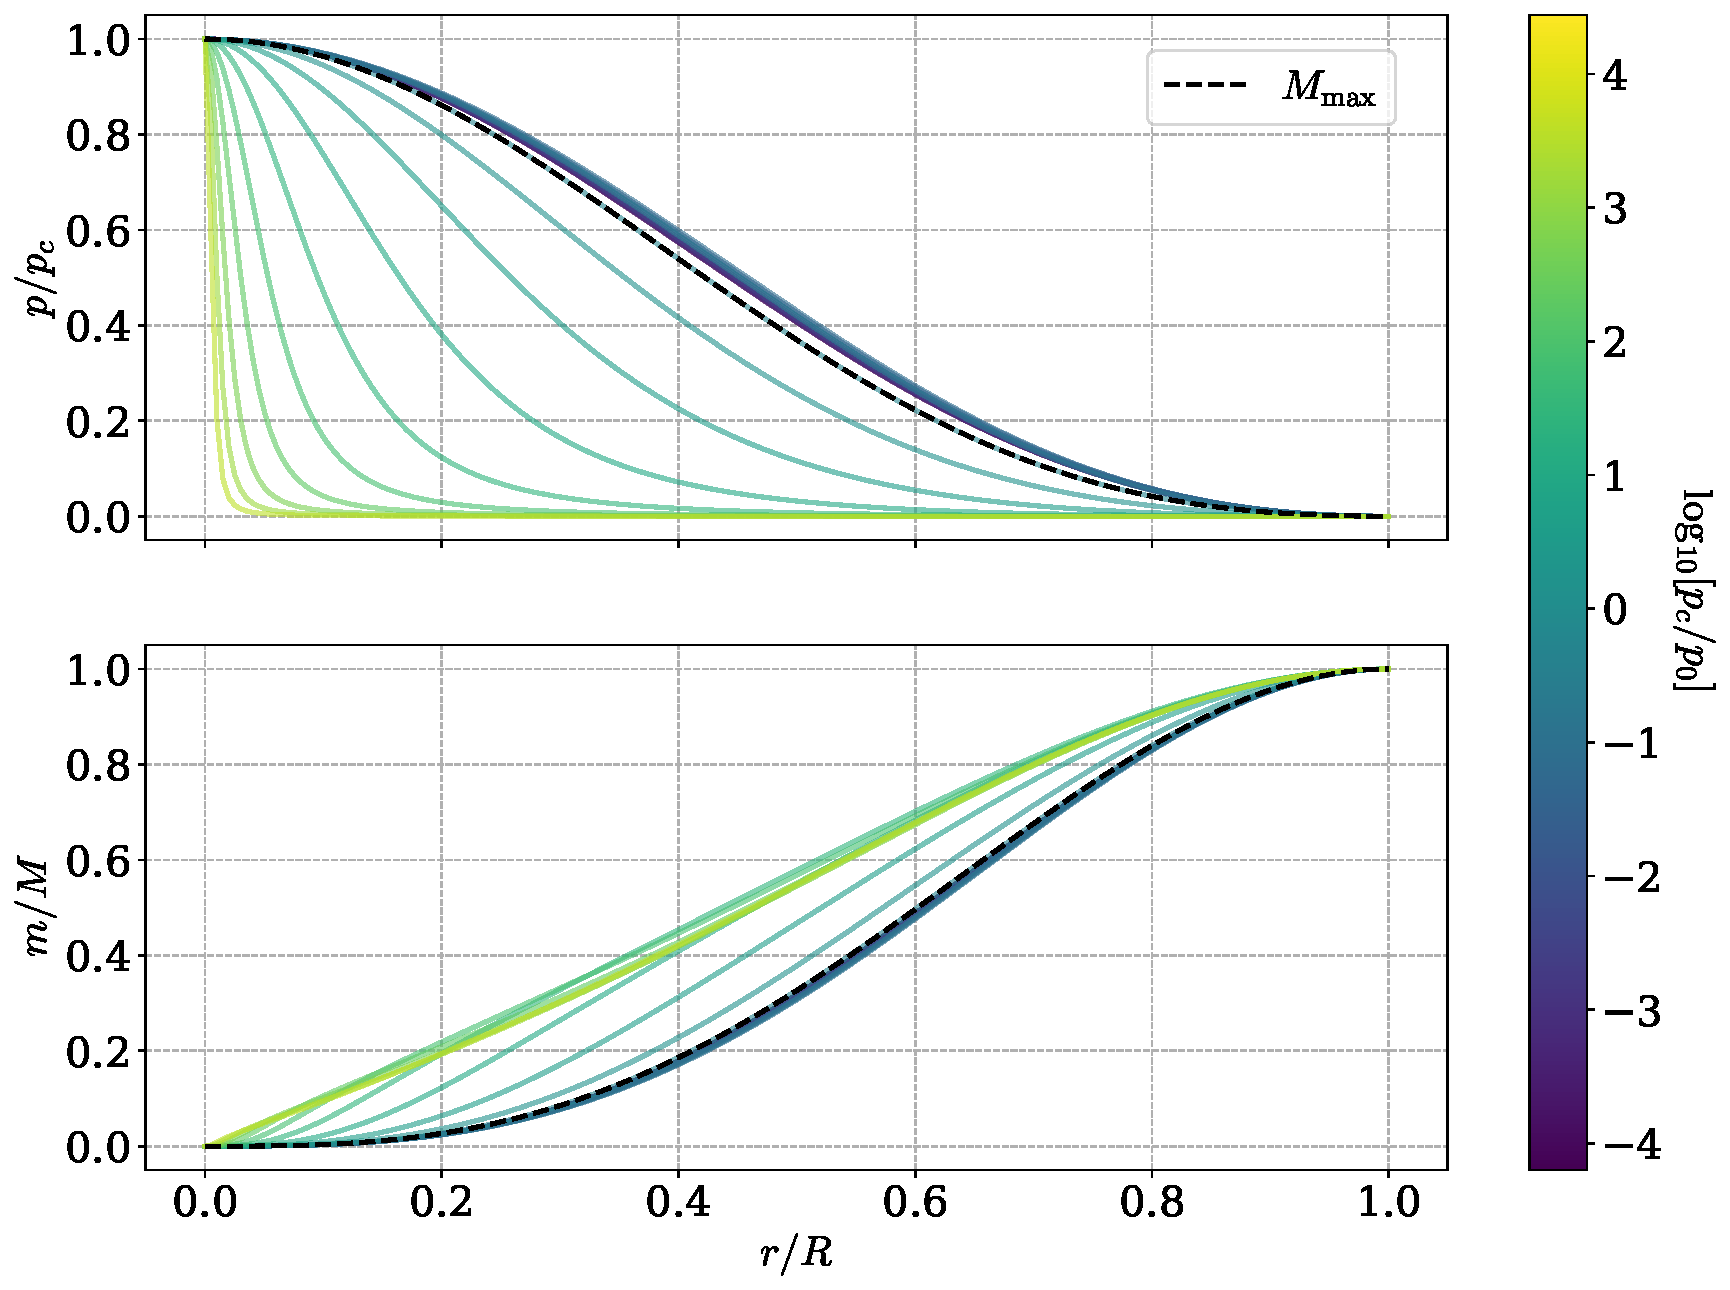
\includegraphics[width=0.8\textwidth]{../scripts/figurer/pion_star/pressure_mass_pion_star.pdf}
    \caption{
    Top: The pressure normalized to the central pressure, as a function of radius, normalized to the stellar radius.
    Bottom: The mass, normalized to the stellar mass, within a radius $r$, normalized to the stellar radius.
    Both plots show a range of stars with different central pressures, indicated by the color.
    The black dashed line corresponds to the star with the largest mass.
    }
    \label{fig: pressure and mass for pion star}
\end{figure}

\begin{figure}[!h]
    \centering
    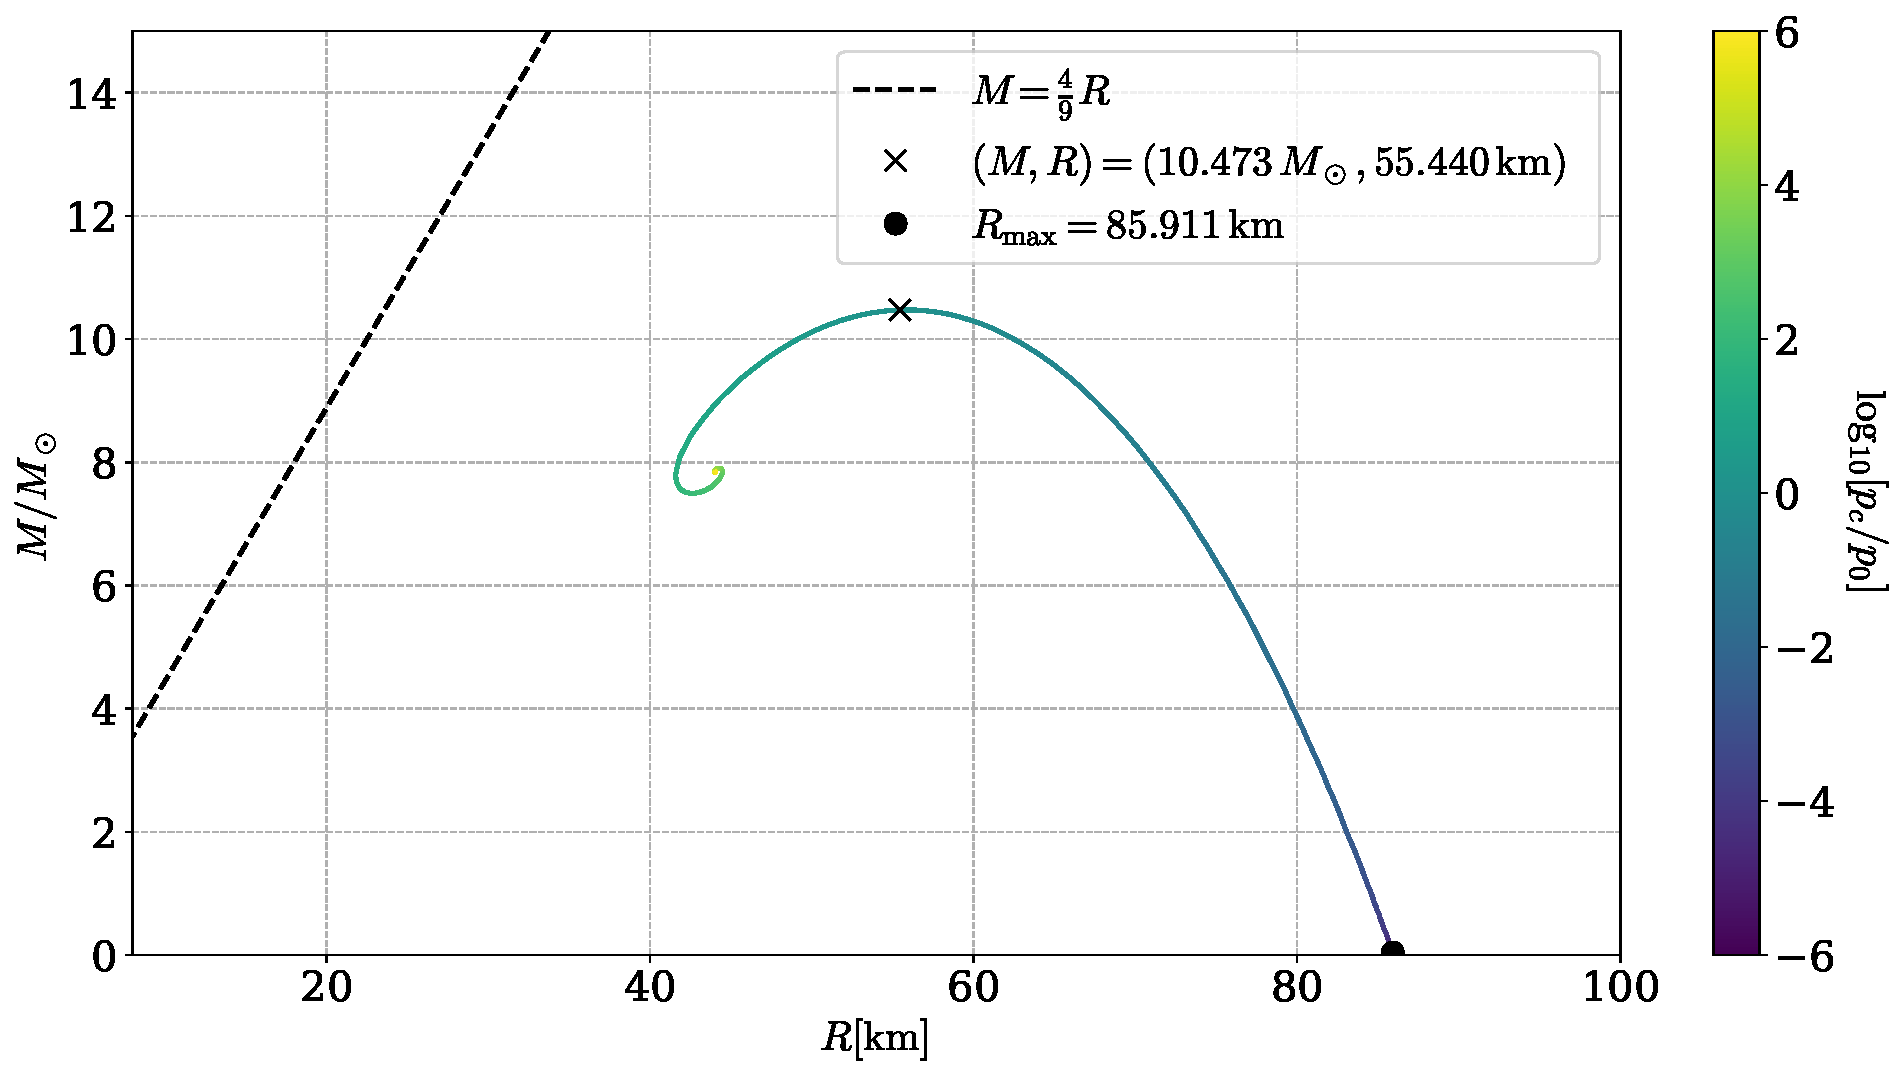
\includegraphics[width=0.85\textwidth]{../scripts/figurer/pion_star/mass_radius_pion_star.pdf}
    \caption{
        The lowest order mass-radius relation a pion star using two-flavor chiral perturbation theory.
        The mass is given in units of solar masses, while the radius is measured in kilometers.
        This line is parameterized by the central pressure $p_c$ of the star, as indicated by the color gradient.
        The dashed black line indicates the theoretical maximum mass for a given radius, and any configuration above it will collapse to a black hole.
        }
        \label{fig: mass-radius relation pion star}
\end{figure}

\begin{figure}[!h]
    \centering
    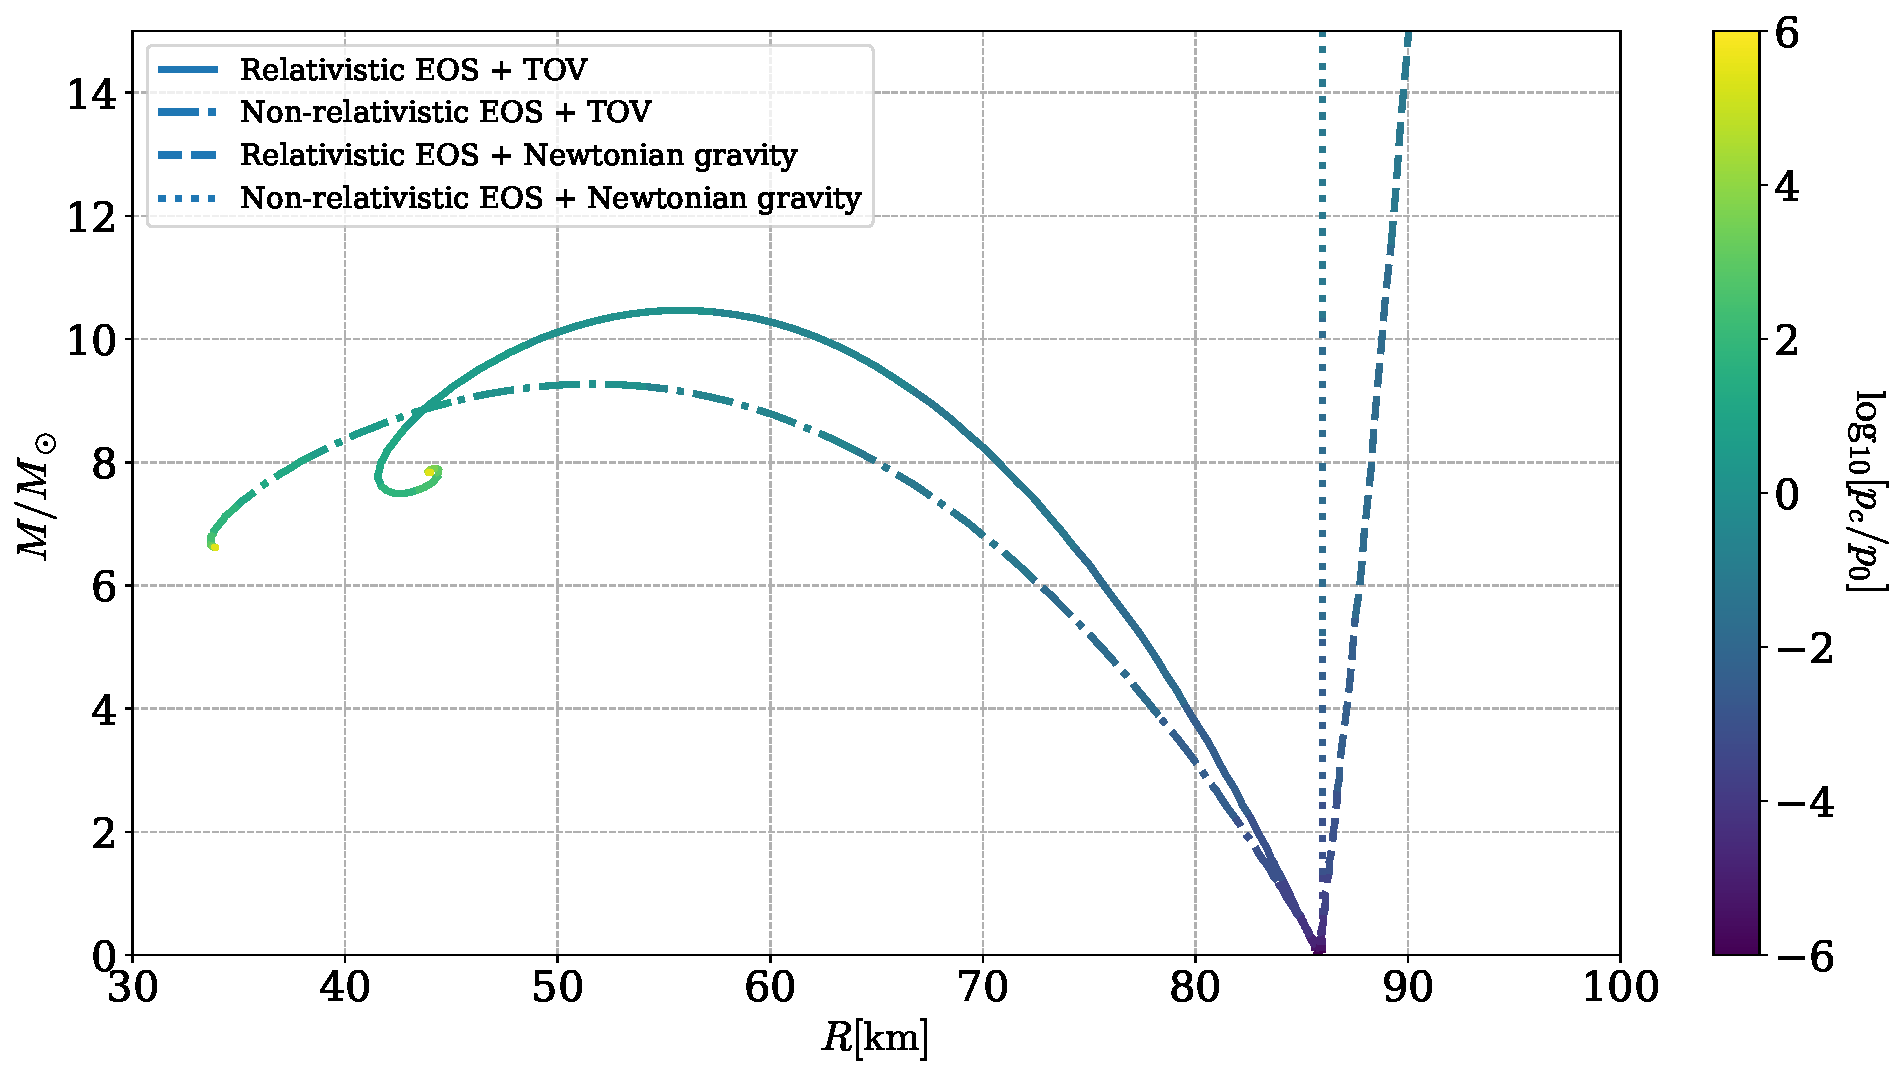
\includegraphics[width=0.85\textwidth]{../scripts/figurer/pion_star/mass_radius_comparison.pdf}
    \caption{
        The mass-radius relationship of the pion star from the full, leading-order equation of state from two-flavor chiral perturbation and the TOV equation, compared with results in various limits.
        }
        \label{fig: mass-radius relation pion star comparison}
\end{figure}


\autoref{fig: mass-radius relation pion star} shows the mass-radius relation for the pion star.
As in the case of the neutron star, it has a maximum mass, in this case of $M_\text{max} = 10.47\, M_\odot$.
However, in contrast to the case of the neutron star, the stellar radius approaches a maximum radius as the central pressure decreases.
This matches our expectation from the non-relativistic, Newtonian limit.
We see that the largest radius in our results, corresponding to  $p_c = 10^{-6} \, p_0$, is $R = 85.82 \, \text{km}$, which is in good agreement with our earlier analysis, \autoref{radius pion star nr limit}.

\autoref{fig: mass-radius relation pion star comparison} compares the mass-radius relation from the full equation of state and TOV equation with various limits.
In the non-relativistic, Newtonian limit, the stellar radius is independent of the mass, as we found in our earlier analysis.

\todo[inline]{Vis kjemisk potensial}



\FloatBarrier
\subsection{Including electromagnetic contributions}


With the results from\autoref{subsection: including electromagnetism lo eos}, the radius of the polytrope and the limiting radius of the full system changes and is now
%
\begin{equation}
    \label{maximum mass pion star with em interaction}
    R = \frac{\pi}{\sqrt{12}(1 + \Delta)} r_0 = 80.40 \, \text{km}.
\end{equation}


\autoref{fig: pressure and energy with EM interaction} shows the pressure and energy density, normalized to their characteristic quantities, as a function of chemical potential above the critical value, normalized to $\bar m$.
\autoref{fig: eos chpt em interaction} shows the equation of state.
The results with and without electromagnetic results are compared.
We see that the inclusion of electromagnetic contributions results in a less stiff equation of state; a given pressure correspond to a higher energy density when including electromagnetic interactions.

\autoref{fig: mass-radius relation leading order pion star with em interaction} shows the mass-radius reaction of the pion star when the electromagnetic interaction is taken into account.
We see that the shape of the curve has not changed much from our earlier result. 
Both the maximum mass and radius are slightly smaller.
The new result for maximum radius, $R_\text{max} = 80.35 \, \text{km}$, is in excellent agreement with our expectation, \autoref{maximum mass pion star with em interaction}.
The result with and without electromagnetic interaction is compared in \autoref{fig: mass-radius relation comparison}.
As discussed in \autoref{section: cold fermi star}, we expect a stiffer equation of state to correspond to a more massive star, as happens in this case.

\begin{figure}[!htb]
    \centering
    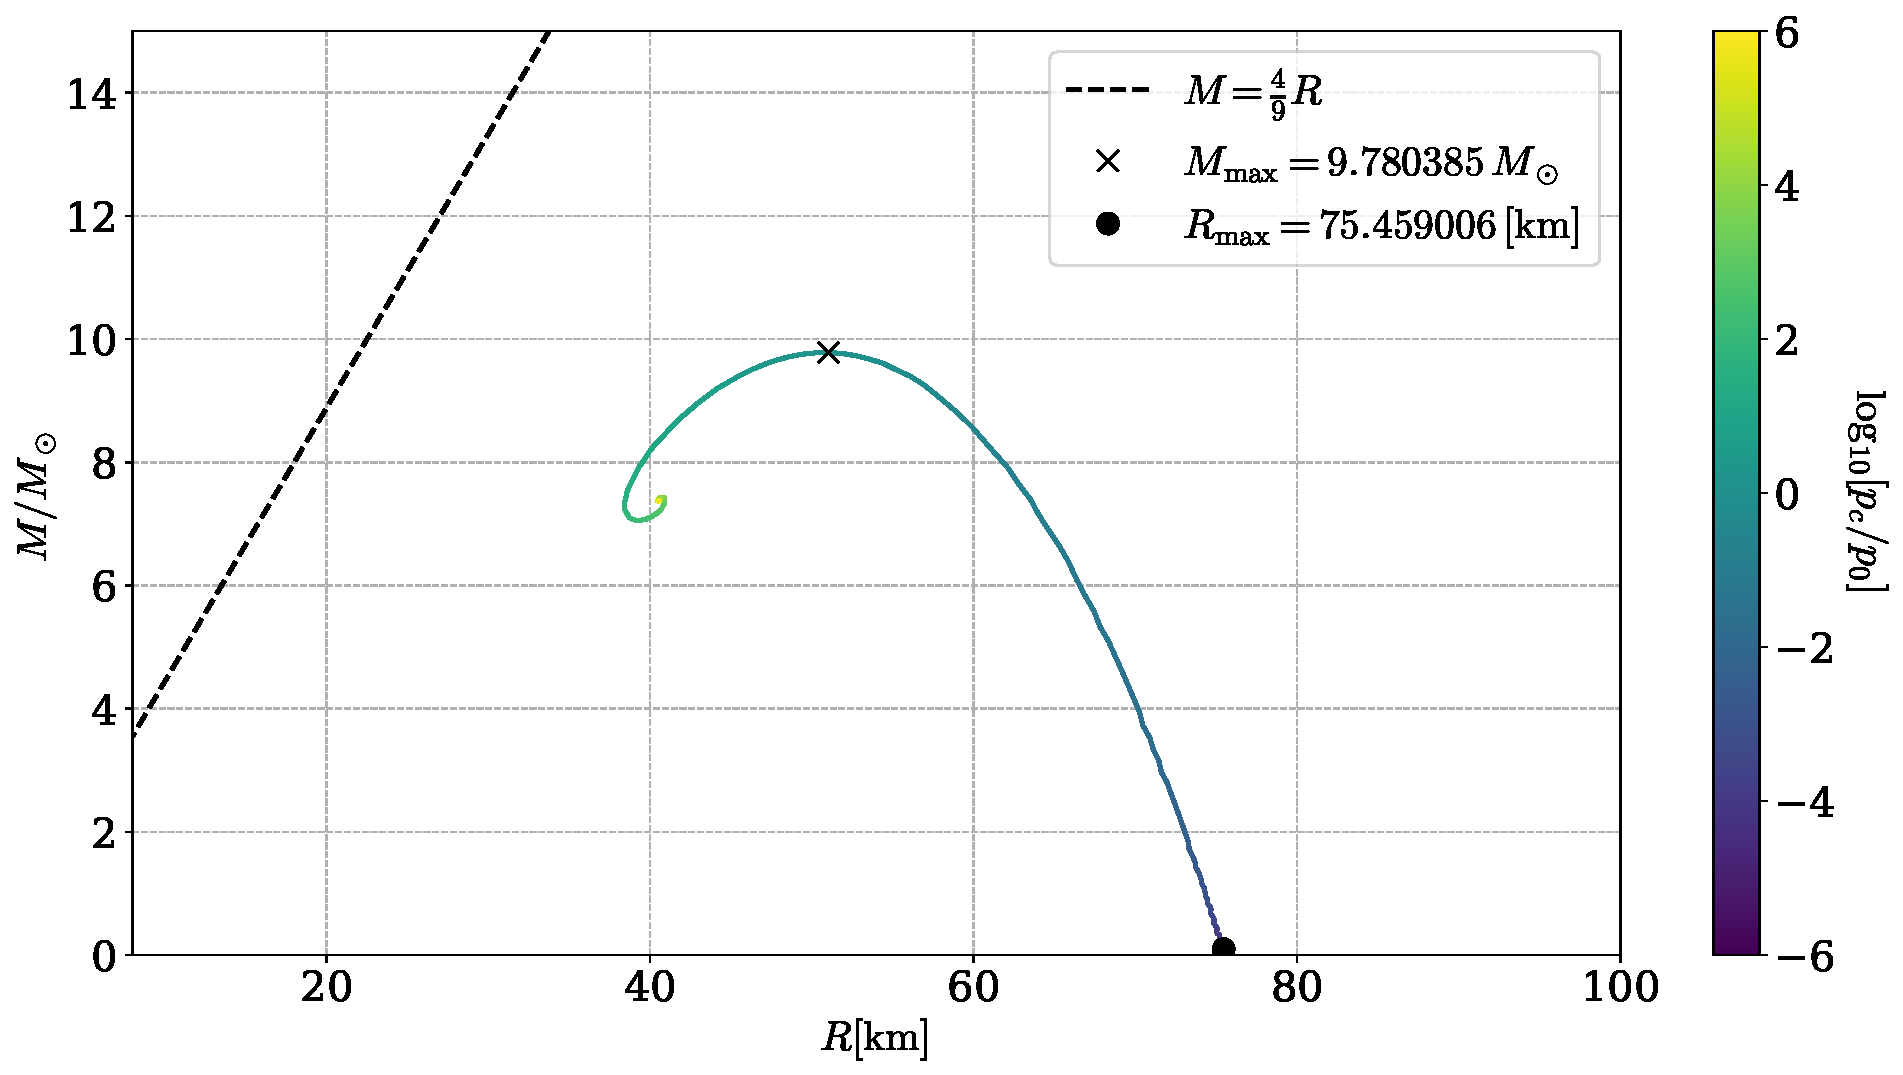
\includegraphics[width=0.85\textwidth]{../scripts/figurer/pion_star/mass_radius_pion_star_EM.pdf}
    \caption{
        The mass-radius relation of a pion star including electromagnetic interactions, parameterized by the logarithm of the central pressure.
        The dashed line shows the absolute limiting mass for a given radius.
        The cross indicates the maximum mass configuration, and the dot the maximum radius configuration.
        The mass is given in units of solar masses, while the radius is in kilometers.
        }
    \label{fig: mass-radius relation leading order pion star with em interaction}
\end{figure}


\begin{figure}[!htb]
    \centering
    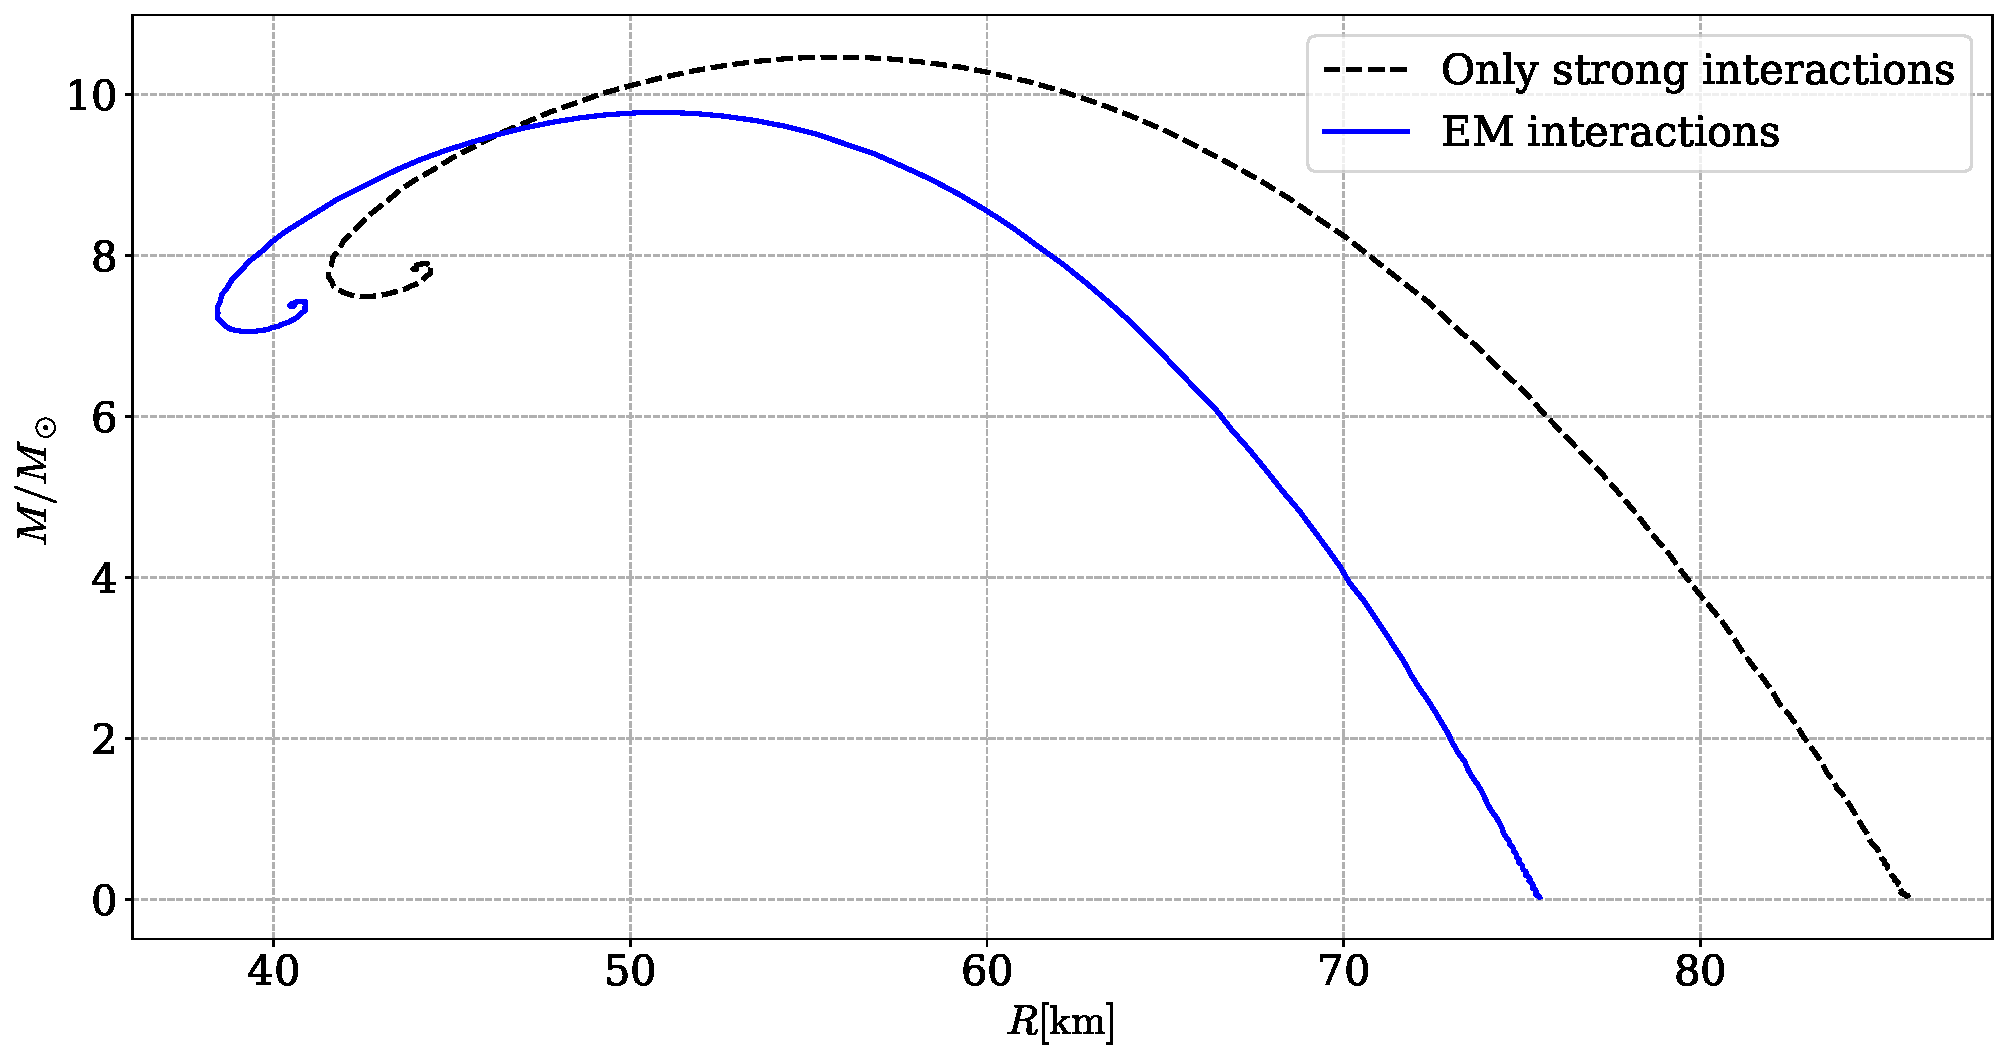
\includegraphics[width=0.85\textwidth]{../scripts/figurer/pion_star/mass_radius_pion_star_compare.pdf}
    \caption{
        The mass-radius relation of pion stars with and without the inclusion of electromagnetism.
        The radius is in km, and the mass in units of the solar mass.
        The marked points are the maximum mass and corresponding radius of the stars.
        }
        \label{fig: mass-radius relation comparison}
\end{figure}

\clearpage

\subsection{Charge neutral stars}


We now apply the results including the constraints of charge neutrality.
The mass-radius relation for pion stars where we include a charged lepton, as discussed in \autoref{section: charge neturality}, is shown in \autoref{fig: mass radius relation with leptons}, and is compared to the relation for pion stars of only pions.
The smaller star is due to the inclusion of the muon, while the larger is from including the electron.
We see that the two leptons affect the relation in different ways.
The light electron does not contribute much to the energy density and the ultrarelativistic limit of the full equation of state quickly approaches that of only the pion. The maximum mass is therefore not changed much, and the corresponding radius is only slightly larger.
In the non-relativisitic regime, however, the electron results in a stiffer equation, and a different polytropic index.
As expected, there is therefore no upper limit to the radius, which only grows with lower total mass and central pressure.
The maximum mass is $ 10.42\, M_\odot $, and the corresponding maximum radius is $59.84\,\text{km}$.
This is slightly less massive and larger than the star of only pions.

The muon, on the other hand, is much heavier and thus mostly contributes to the energy density.
This results in a less stiff equation of state, and a smaller and less massive star.
The maximum mass is $ 5.970\, M_\odot $, and the corresponding maximum radius is $31.52\,\text{km}$.
As discussed, the equation of state here admits an intermediate limit over a large interval, where it behaves as a polytrope with $\gamma = 2$.
As this is such a good approximation for the equation of state, the mass-radius relation seems to approach a maximum radius.
Similarly to what happens with the inclusion of electromagnetic interaction, the polytrope constant $K$ is modified to $K^{-1} = 8 (1 + \Delta_\ell)^2$, where
%
\begin{equation}
    \Delta_\ell = \frac{4}{3} \frac{u_{\ell, 0}}{u_0} A^{-1}.
\end{equation}
%
In the case of the muon, this leads to a modified maximum radius,
%
\begin{equation}
    R = \frac{\pi}{\sqrt{12} (1 + \Delta_\mu)} = 42.64\, \text{km}.
\end{equation}
%
From \autoref{fig: mass radius relation with leptons}, we see that this fits well with the numerical results.
This limit is, however, only intermediate, and we should expect that as the central pressure falls even further, the radius will start to grow without bounds.
Indeed, we can notice a slight curve towards higher radius at the lowest mass.
To demonstrate this effect further, we would need much higher precision numerical computation, and furthermore it would take us to regime where other approximations such as zero temperature become dubious.


\begin{figure}[!htb]
    \centering
    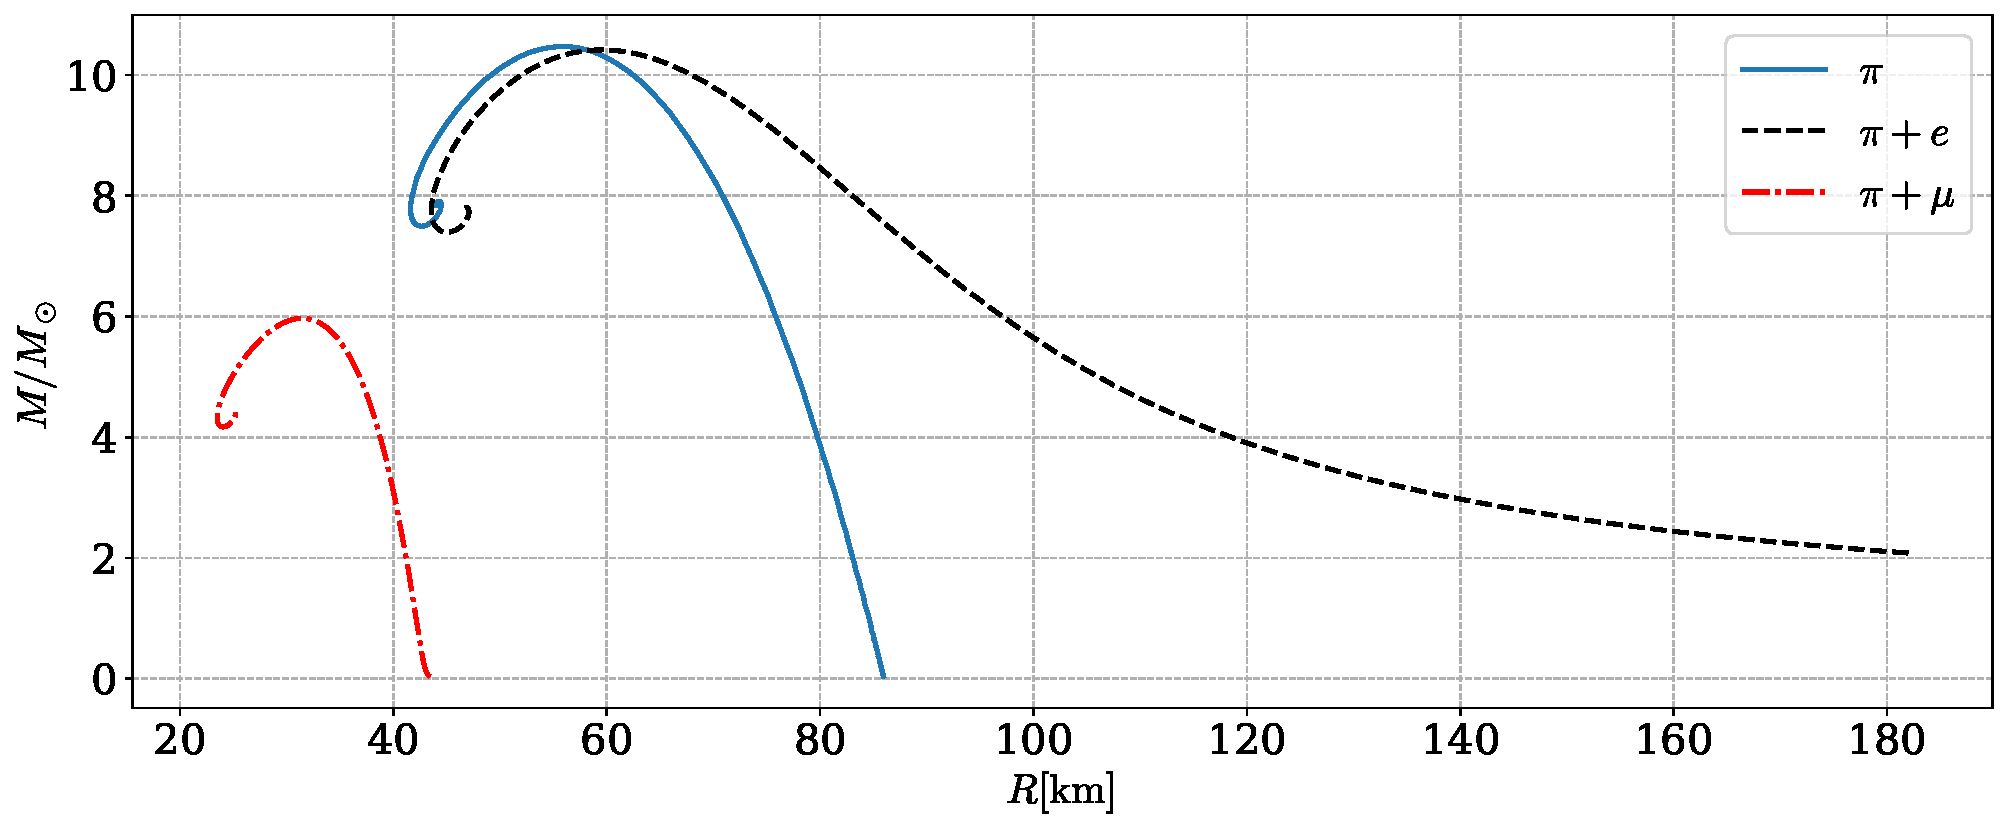
\includegraphics[width=\textwidth]{../scripts/figurer/pion_star/mass_radius_lepton.pdf}
    \caption{
        The mass-radius relation of pion stars, with and without a lepton to enforce charge neutrality.
        The radius is given in km, and the mass in solar masses.
        }
        \label{fig: mass radius relation with leptons}
\end{figure}



